\chapter{OFDM \& Multicarrier Modulation}
\label{ch:ofdm}

\begin{nontechnical}
\textbf{OFDM is like splitting a highway into many lanes}---if one lane has an accident (interference), the other lanes keep traffic flowing!

\textbf{The problem OFDM solves:}
\begin{itemize}
\item Sending data fast on one channel = short pulses = easily disrupted by echoes/reflections
\item It's like trying to drive 100 mph on a narrow road---one pothole ruins everything!
\end{itemize}

\textbf{The OFDM solution:}
\begin{itemize}
\item Split data across \textbf{hundreds or thousands} of narrow ``lanes'' (subcarriers)
\item Each lane moves slowly (easier to handle)
\item If one lane fades or gets interference, you still have 999 others working!
\end{itemize}

\textbf{Real-world example---WiFi:}
\begin{itemize}
\item \textbf{WiFi 5 (802.11ac):} Uses 52--468 subcarriers
\item \textbf{WiFi 6 (802.11ax):} Uses up to 1960 subcarriers!
\item Each subcarrier is only 78 kHz wide (vs 20--160 MHz total channel)
\item Like delivering packages: 1 huge truck (risky!) vs 100 small vans (resilient!)
\end{itemize}

\textbf{Why it's everywhere:}
\begin{itemize}
\item \textbf{WiFi:} All modern WiFi uses OFDM
\item \textbf{4G/5G:} LTE and 5G NR are OFDM-based
\item \textbf{Digital TV:} DVB-T uses OFDM for broadcast
\item \textbf{DSL:} Even wired broadband uses OFDM (DMT variant)!
\end{itemize}

\textbf{Fun fact:} OFDM uses a clever math trick (FFT) to pack subcarriers so tightly they overlap without interfering---it's called ``orthogonality'' (like fingers interlaced).
\end{nontechnical}

\section{Overview}

\textbf{Orthogonal Frequency-Division Multiplexing (OFDM)} is a multicarrier modulation technique that divides a wideband channel into many narrow, orthogonal subcarriers. It has become the dominant physical layer technology in modern wireless and wireline communications.

\begin{keyconcept}
OFDM converts a \textbf{frequency-selective fading channel} into many parallel \textbf{flat-fading channels}. Each subcarrier experiences approximately constant gain and phase across its narrow bandwidth, dramatically simplifying equalization.
\end{keyconcept}

OFDM forms the foundation for:
\begin{itemize}
\item \textbf{WiFi:} 802.11a/g/n/ac/ax/be (all variants since 1999)
\item \textbf{4G LTE:} All downlink and uplink transmissions
\item \textbf{5G NR:} Scalable numerology OFDM with flexible subcarrier spacing
\item \textbf{Digital TV:} DVB-T/T2, ISDB-T, ATSC 3.0
\item \textbf{DSL:} Discrete Multitone (DMT) for ADSL/VDSL
\end{itemize}

\section{Mathematical Description}

\subsection{The Core Problem: Multipath and ISI}

\textbf{Single-carrier problem:} High-speed data requires short symbol duration, making signals susceptible to intersymbol interference (ISI) from multipath propagation.

For a data rate $R_b$ with symbol duration:
\begin{equation}
T_s = \frac{1}{R_s}
\end{equation}
where:
\begin{itemize}
\item $T_s$ = symbol duration (seconds)
\item $R_s$ = symbol rate (symbols/second)
\end{itemize}

\textbf{ISI criterion:} When delay spread $\tau_{\mathrm{RMS}} > 0.1 T_s$, severe ISI occurs.

\textbf{OFDM solution:} Divide spectrum into $N$ narrow subcarriers. Each subcarrier symbol duration:
\begin{equation}
T_{\mathrm{OFDM}} = N \cdot T_s
\end{equation}

Since $T_{\mathrm{OFDM}} \gg T_s$, the condition $\tau_{\mathrm{RMS}} \ll T_{\mathrm{OFDM}}$ is easily satisfied.

\subsection{Orthogonality Condition}

The fundamental principle of OFDM is that subcarriers are \textbf{orthogonal}---they can overlap in frequency without interfering.

Subcarrier frequencies are defined as:
\begin{equation}
f_k = f_c + k \cdot \Delta f
\end{equation}
where:
\begin{itemize}
\item $f_c$ = center frequency (Hz)
\item $k$ = subcarrier index $(0, 1, 2, \ldots, N-1)$
\item $\Delta f = \frac{1}{T_u}$ = subcarrier spacing (Hz)
\item $T_u$ = useful OFDM symbol duration (seconds)
\end{itemize}

\textbf{Orthogonality integral:} Over one symbol period $T_u$, the correlation between different subcarriers is zero:
\begin{equation}
\int_0^{T_u} e^{j2\pi f_k t} \cdot e^{-j2\pi f_m t} \, dt = \begin{cases}
T_u & \text{if } k = m \\
0 & \text{if } k \neq m
\end{cases}
\end{equation}

This ensures subcarriers don't interfere despite \textbf{spectral overlap}---a key efficiency advantage.

\subsection{IFFT/FFT Implementation}

\textbf{Key insight:} OFDM modulation/demodulation is mathematically equivalent to Inverse Fast Fourier Transform (IFFT) and FFT operations.

\textbf{Transmitter (IFFT):}
\begin{equation}
x[n] = \frac{1}{\sqrt{N}} \sum_{k=0}^{N-1} X_k \cdot e^{j2\pi kn/N}, \quad n = 0, 1, \ldots, N-1
\end{equation}
where:
\begin{itemize}
\item $X_k$ = complex data symbol on subcarrier $k$ (from QAM/PSK constellation)
\item $x[n]$ = time-domain OFDM sample
\item $N$ = FFT size (typically 64, 128, 256, 512, 1024, 2048, 4096)
\end{itemize}

\textbf{Receiver (FFT):}
\begin{equation}
Y_k = \frac{1}{\sqrt{N}} \sum_{n=0}^{N-1} y[n] \cdot e^{-j2\pi kn/N}, \quad k = 0, 1, \ldots, N-1
\end{equation}
where:
\begin{itemize}
\item $y[n]$ = received time-domain samples (after cyclic prefix removal)
\item $Y_k$ = recovered symbol on subcarrier $k$
\end{itemize}

\begin{calloutbox}{Computational Advantage}
The FFT algorithm reduces computational complexity from $O(N^2)$ to $O(N \log_2 N)$.

\textbf{Example:} For $N = 1024$ subcarriers:
\begin{itemize}
\item Direct DFT: $1{,}024^2 = 1{,}048{,}576$ complex multiplications
\item FFT: $1{,}024 \cdot \log_2(1{,}024) = 10{,}240$ complex multiplications
\item \textbf{Speedup:} $100\times$ faster!
\end{itemize}

This makes real-time OFDM practical on low-power digital signal processors.
\end{calloutbox}

\section{Modulation and Demodulation}

\subsection{Frequency Domain Visualization}

OFDM subcarriers overlap in frequency but remain orthogonal:

\begin{center}
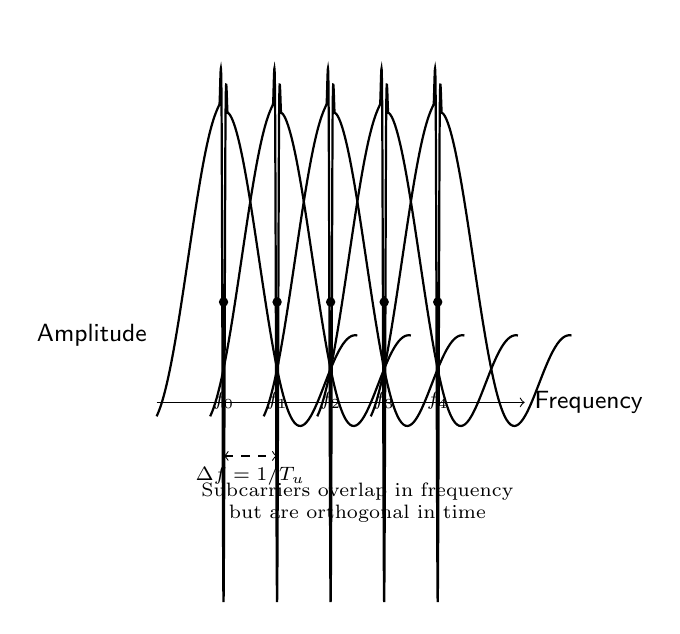
\begin{tikzpicture}[scale=0.85]
% Draw 5 overlapping subcarrier sinc functions
\foreach \k in {0,1,2,3,4} {
  \draw[domain=-1+\k*0.8:2+\k*0.8, samples=100, smooth, thick] 
    plot (\x, {sin((\x-\k*0.8)*180/0.8)/(\x-\k*0.8+0.001)});
  % Peak markers
  \fill[black] (\k*0.8, 1) circle (2pt);
  % Frequency labels
  \node[below,font=\scriptsize] at (\k*0.8, -0.2) {$f_{\k}$};
}

% Axes
\draw[->] (-1,-0.5) -- (4.5,-0.5) node[right,font=\sffamily\small] {Frequency};
\node[left,font=\sffamily\small] at (-1,0.5) {Amplitude};

% Spacing annotation
\draw[<->,dashed] (0,-1.3) -- (0.8,-1.3) node[midway,below,font=\scriptsize] {$\Delta f = 1/T_u$};

% Orthogonality note
\node[align=center,font=\scriptsize] at (2,-2) {Subcarriers overlap in frequency\\but are orthogonal in time};
\end{tikzpicture}
\end{center}

\textbf{Key observation:} At each subcarrier's center frequency, all other subcarriers have zero amplitude (nulls). This is the essence of orthogonality.

\subsection{Transmitter (Modulator)}

\begin{center}
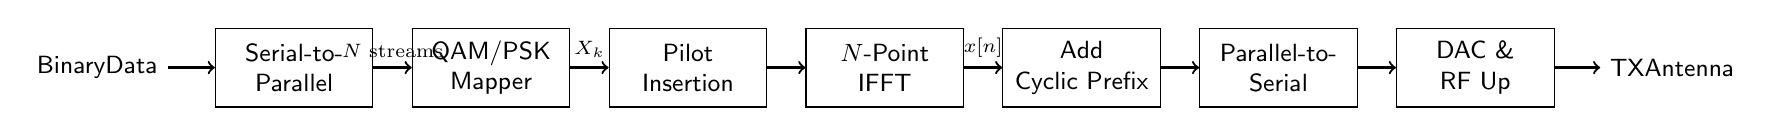
\begin{tikzpicture}[
  block/.style={rectangle, draw, minimum width=2cm, minimum height=1cm, font=\sffamily\small, align=center},
  node distance=1.8cm,
  font=\small
]
\node (input) {\sffamily Binary\\Data};
\node[block, right of=input, node distance=2.5cm] (s2p) {Serial-to-\\Parallel};
\node[block, right of=s2p, node distance=2.5cm] (map) {QAM/PSK\\Mapper};
\node[block, right of=map, node distance=2.5cm] (pilot) {Pilot\\Insertion};
\node[block, right of=pilot, node distance=2.5cm] (ifft) {$N$-Point\\IFFT};
\node[block, right of=ifft, node distance=2.5cm] (cp) {Add\\Cyclic Prefix};
\node[block, right of=cp, node distance=2.5cm] (p2s) {Parallel-to-\\Serial};
\node[block, right of=p2s, node distance=2.5cm] (dac) {DAC \&\\RF Up};
\node[right of=dac, node distance=2.5cm] (ant) {\sffamily TX\\Antenna};

% Arrows
\draw[->,thick] (input) -- (s2p);
\draw[->,thick] (s2p) -- node[above,font=\scriptsize] {$N$ streams} (map);
\draw[->,thick] (map) -- node[above,font=\scriptsize] {$X_k$} (pilot);
\draw[->,thick] (pilot) -- (ifft);
\draw[->,thick] (ifft) -- node[above,font=\scriptsize] {$x[n]$} (cp);
\draw[->,thick] (cp) -- (p2s);
\draw[->,thick] (p2s) -- (dac);
\draw[->,thick] (dac) -- (ant);
\end{tikzpicture}
\end{center}

\textbf{Process:}
\begin{enumerate}
\item \textbf{Serial-to-Parallel:} Incoming bit stream is split into $N$ parallel streams
\item \textbf{Symbol Mapping:} Each stream is mapped to QAM/PSK constellation (e.g., QPSK, 16-QAM, 64-QAM)
\item \textbf{Pilot Insertion:} Known symbols inserted on pilot subcarriers for channel estimation
\item \textbf{IFFT:} Converts frequency-domain symbols $X_k$ to time-domain samples $x[n]$
\item \textbf{Cyclic Prefix:} Last $L_{\mathrm{CP}}$ samples copied to beginning of symbol
\item \textbf{Parallel-to-Serial:} Convert to serial stream for transmission
\item \textbf{DAC \& RF Upconversion:} Digital-to-analog conversion and carrier modulation
\end{enumerate}

\subsection{Receiver (Demodulator)}

\begin{center}
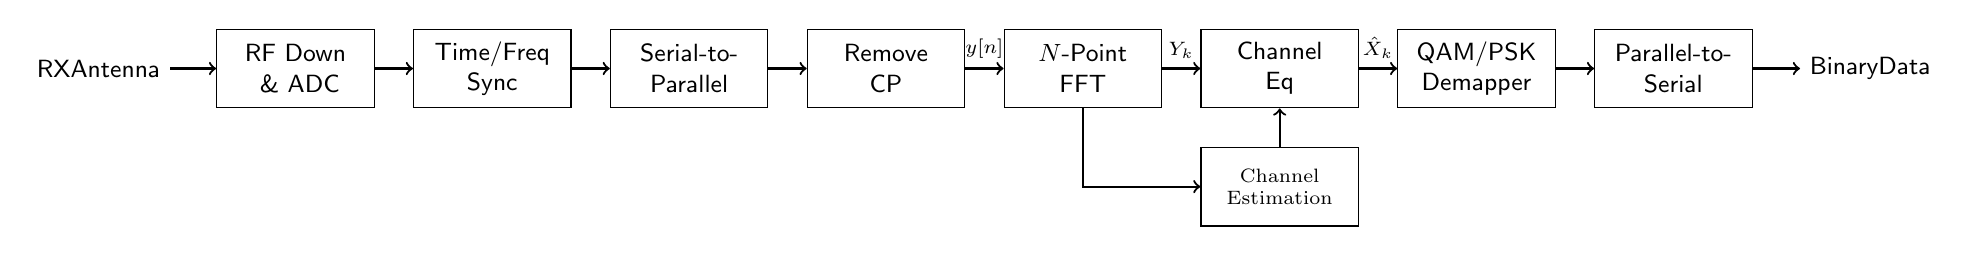
\begin{tikzpicture}[
  block/.style={rectangle, draw, minimum width=2cm, minimum height=1cm, font=\sffamily\small, align=center},
  node distance=1.8cm,
  font=\small
]
\node (ant) {\sffamily RX\\Antenna};
\node[block, right of=ant, node distance=2.5cm] (adc) {RF Down\\\ \& ADC};
\node[block, right of=adc, node distance=2.5cm] (sync) {Time/Freq\\Sync};
\node[block, right of=sync, node distance=2.5cm] (s2p) {Serial-to-\\Parallel};
\node[block, right of=s2p, node distance=2.5cm] (cpr) {Remove\\CP};
\node[block, right of=cpr, node distance=2.5cm] (fft) {$N$-Point\\FFT};
\node[block, right of=fft, node distance=2.5cm] (eq) {Channel\\Eq};
\node[block, right of=eq, node distance=2.5cm] (demap) {QAM/PSK\\Demapper};
\node[block, right of=demap, node distance=2.5cm] (p2s) {Parallel-to-\\Serial};
\node[right of=p2s, node distance=2.5cm] (output) {\sffamily Binary\\Data};

% Arrows
\draw[->,thick] (ant) -- (adc);
\draw[->,thick] (adc) -- (sync);
\draw[->,thick] (sync) -- (s2p);
\draw[->,thick] (s2p) -- (cpr);
\draw[->,thick] (cpr) -- node[above,font=\scriptsize] {$y[n]$} (fft);
\draw[->,thick] (fft) -- node[above,font=\scriptsize] {$Y_k$} (eq);
\draw[->,thick] (eq) -- node[above,font=\scriptsize] {$\hat{X}_k$} (demap);
\draw[->,thick] (demap) -- (p2s);
\draw[->,thick] (p2s) -- (output);

% Channel estimation feedback
\node[block, below of=eq, node distance=1.5cm, font=\scriptsize] (chest) {Channel\\Estimation};
\draw[->,thick] (fft) |- (chest);
\draw[->,thick] (chest) -- (eq);
\end{tikzpicture}
\end{center}

\textbf{Process:}
\begin{enumerate}
\item \textbf{RF Downconversion \& ADC:} Received signal is downconverted and digitized
\item \textbf{Synchronization:} Time and frequency offsets are corrected
\item \textbf{Serial-to-Parallel:} Convert to $N+L_{\mathrm{CP}}$ parallel samples
\item \textbf{Remove CP:} Discard cyclic prefix samples (guard interval)
\item \textbf{FFT:} Convert time-domain $y[n]$ to frequency-domain $Y_k$
\item \textbf{Channel Estimation:} Use pilot subcarriers to estimate $H_k$ for each subcarrier
\item \textbf{Equalization:} One-tap equalizer per subcarrier: $\hat{X}_k = Y_k / H_k$
\item \textbf{Demapping:} Recover bits from constellation symbols
\item \textbf{Parallel-to-Serial:} Reconstruct original bit stream
\end{enumerate}

\begin{warningbox}
\textbf{Synchronization is critical in OFDM.} Carrier frequency offset (CFO) destroys orthogonality between subcarriers, causing inter-carrier interference (ICI). A CFO of just $1\%$ of subcarrier spacing can degrade performance by several dB. Robust synchronization algorithms (Schmidl-Cox, etc.) are essential.
\end{warningbox}

\section{Cyclic Prefix}

The \textbf{cyclic prefix} is OFDM's critical defense mechanism against multipath-induced intersymbol interference.

\subsection{Cyclic Prefix Construction}

The cyclic prefix consists of the \textbf{last $L_{\mathrm{CP}}$ samples} of the OFDM symbol, copied and prepended to the symbol:
\begin{equation}
x_{\mathrm{CP}}[n] = \begin{cases}
x[N + n] & \text{for } n = -L_{\mathrm{CP}}, \ldots, -1 \text{ (CP)} \\
x[n] & \text{for } n = 0, 1, \ldots, N-1 \text{ (original symbol)}
\end{cases}
\end{equation}

Total transmitted samples per OFDM symbol:
\begin{equation}
N_{\mathrm{total}} = N + L_{\mathrm{CP}}
\end{equation}

\textbf{Visual representation:}
\begin{center}
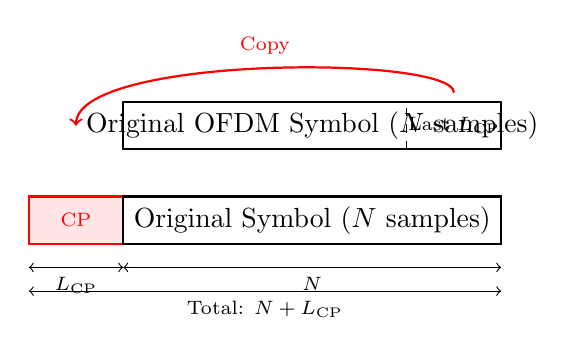
\begin{tikzpicture}[scale=0.6]
% Original symbol
\draw[thick] (0,0) rectangle (8,1);
\node at (4,0.5) {Original OFDM Symbol ($N$ samples)};
\draw[dashed] (6,0) -- (6,1);
\node[font=\scriptsize] at (7,0.5) {Last $L_{\mathrm{CP}}$};

% Arrow indicating copy
\draw[->,thick,red] (7,1.2) .. controls (7,2) and (-1,2) .. (-1,0.5);
\node[red,font=\scriptsize] at (3,2.2) {Copy};

% With CP
\draw[thick,red,fill=red!10] (-2,-2) rectangle (0,-1);
\draw[thick] (0,-2) rectangle (8,-1);
\node[red,font=\scriptsize] at (-1,-1.5) {CP};
\node at (4,-1.5) {Original Symbol ($N$ samples)};

\draw[<->] (-2,-2.5) -- (0,-2.5) node[midway,below,font=\scriptsize] {$L_{\mathrm{CP}}$};
\draw[<->] (0,-2.5) -- (8,-2.5) node[midway,below,font=\scriptsize] {$N$};
\draw[<->] (-2,-3) -- (8,-3) node[midway,below,font=\scriptsize] {Total: $N + L_{\mathrm{CP}}$};
\end{tikzpicture}
\end{center}

\subsection{Why Cyclic Prefix Works}

\textbf{Problem:} Multipath creates delayed copies of the signal, causing samples from adjacent symbols to overlap (ISI).

\textbf{Solution:} The CP acts as a \textbf{guard interval}:
\begin{itemize}
\item If delay spread $\tau_{\mathrm{max}} < T_{\mathrm{CP}}$, ISI from previous symbol falls entirely within the CP
\item Receiver discards CP samples, keeping only clean symbol data
\item CP converts \textbf{linear convolution into circular convolution}, enabling simple per-subcarrier equalization
\end{itemize}

\textbf{Mathematical insight:} With CP, the received signal on subcarrier $k$ is:
\begin{equation}
Y_k = H_k \cdot X_k + N_k
\end{equation}
where:
\begin{itemize}
\item $H_k$ = complex channel gain on subcarrier $k$
\item $X_k$ = transmitted symbol on subcarrier $k$
\item $N_k$ = noise on subcarrier $k$
\end{itemize}

This allows \textbf{one-tap equalization} per subcarrier:
\begin{equation}
\hat{X}_k = \frac{Y_k}{H_k} = X_k + \frac{N_k}{H_k}
\end{equation}

\subsection{CP Overhead and Design Trade-offs}

CP reduces spectral efficiency. The overhead is:
\begin{equation}
\mathrm{Overhead} = \frac{L_{\mathrm{CP}}}{N + L_{\mathrm{CP}}}
\end{equation}

\textbf{Example---WiFi 802.11a:}
\begin{itemize}
\item $N = 64$ subcarriers
\item $L_{\mathrm{CP}} = 16$ samples
\item Overhead = $\frac{16}{80} = 20\%$ spectral efficiency loss
\end{itemize}

\textbf{Trade-off:}
\begin{itemize}
\item[\checkmark] Longer CP $\rightarrow$ more robust to delay spread (better ISI immunity)
\item[\texttimes] Longer CP $\rightarrow$ higher overhead (lower data rate)
\end{itemize}

\textbf{CP length criterion:}
\begin{equation}
L_{\mathrm{CP}} > \tau_{\mathrm{max}} \cdot f_s
\end{equation}
where:
\begin{itemize}
\item $\tau_{\mathrm{max}}$ = maximum expected delay spread (seconds)
\item $f_s$ = sampling frequency (samples/second)
\end{itemize}

\section{OFDM Parameters}

Key design parameters and their relationships:

\begin{center}
\begin{tabular}{@{}llll@{}}
\toprule
\textbf{Parameter} & \textbf{Symbol} & \textbf{Typical Values} & \textbf{Impact} \\
\midrule
FFT Size & $N$ & 64--4096 & Granularity, latency \\
Subcarrier Spacing & $\Delta f$ & 15--240 kHz & Doppler tolerance \\
Symbol Duration & $T_u$ & $1/\Delta f$ & ISI resistance \\
CP Length & $L_{\mathrm{CP}}$ & $N/4$ to $N/16$ & Delay spread tolerance \\
Bandwidth & $BW$ & $N \cdot \Delta f$ & Throughput \\
\bottomrule
\end{tabular}
\end{center}

\textbf{Fundamental relationships:}
\begin{equation}
\Delta f = \frac{1}{T_u}
\end{equation}

\begin{equation}
T_{\mathrm{symbol}} = T_u + T_{\mathrm{CP}}
\end{equation}

\begin{equation}
BW = N_{\mathrm{used}} \cdot \Delta f
\end{equation}
where $N_{\mathrm{used}} \leq N$ (not all subcarriers may be used).

\subsection{Example: LTE (20 MHz)}

\textbf{Configuration:}
\begin{itemize}
\item FFT Size: $N = 2048$
\item Used subcarriers: $N_{\mathrm{used}} = 1200$
\item Subcarrier spacing: $\Delta f = 15$ kHz
\item Symbol duration: $T_u = 66.67$ µs
\item CP (normal): $T_{\mathrm{CP}} = 4.69$ µs (first), $5.21$ µs (others)
\item Bandwidth: $BW = 1200 \times 15 = 18$ MHz
\item Resource blocks: 100 RBs (12 subcarriers $\times$ 180 kHz each)
\item OFDM symbols per slot: 7 symbols = 0.5 ms
\end{itemize}

\section{Pilot Subcarriers and Channel Estimation}

Not all subcarriers carry data---some are \textbf{pilots} for channel estimation and synchronization.

\subsection{Pilot Types}

\textbf{1. Scattered Pilots} (time + frequency diversity for fast fading):
\begin{itemize}
\item Distributed across time and frequency
\item Used in DVB-T, LTE downlink
\end{itemize}

\textbf{2. Continual Pilots} (phase/frequency tracking):
\begin{itemize}
\item Fixed subcarriers always carry pilots
\item Example: WiFi 802.11a uses subcarriers $k = -21, -7, 7, 21$
\end{itemize}

\textbf{3. Preamble/Training Symbols}:
\begin{itemize}
\item First OFDM symbol(s) in a frame contain all pilots
\item Used for initial synchronization and coarse channel estimation
\end{itemize}

\subsection{Channel Estimation Process}

For pilot subcarrier $k_p$, transmitter sends known symbol $P_{k_p}$. Receiver measures:
\begin{equation}
Y_{k_p} = H_{k_p} \cdot P_{k_p} + N_{k_p}
\end{equation}

Channel estimate:
\begin{equation}
\hat{H}_{k_p} = \frac{Y_{k_p}}{P_{k_p}}
\end{equation}

For data subcarriers (non-pilot), $\hat{H}_k$ is obtained by interpolation (linear, spline, or 2D Wiener filtering).

Once channel is estimated, equalization is simply:
\begin{equation}
\hat{X}_k = \frac{Y_k}{\hat{H}_k}
\end{equation}

\begin{calloutbox}{One-Tap Equalization}
OFDM's greatest advantage: Channel equalization reduces to \textbf{one complex division per subcarrier}. Compare this to single-carrier systems requiring complex time-domain equalizers with hundreds of taps and adaptive algorithms. The cyclic prefix converts multipath into a simple frequency-domain multiplication.
\end{calloutbox}

\subsection{\texorpdfstring{ Multipath \& Frequency-Selective
Fading}{ Multipath \& Frequency-Selective Fading}}\label{multipath-frequency-selective-fading}

\subsubsection{Why OFDM Excels in
Multipath}\label{why-ofdm-excels-in-multipath}

\textbf{Single-carrier}: Entire bandwidth experiences
\textbf{frequency-selective fading} \$\textbackslash rightarrow\$ deep
nulls can wipe out signal.

\textbf{OFDM}: Channel appears \textbf{flat} within each narrow
subcarrier \$\textbackslash rightarrow\$ only some subcarriers fade
deeply, others remain strong.

\begin{verbatim}
Frequency Response (Multipath Channel):
Magnitude
    
    |  ___       ___
    | |   |     |   |___       Single-carrier spans entire BW
    | |   |_____|       |        (suffers deep null)
    |_|___|_____________|___ Frequency
                   
       |   |   |   |   |
     OFDM subcarriers (most unaffected, a few degraded)
\end{verbatim}

\textbf{Per-subcarrier equalization}:

\begin{verbatim}
X = Y / H  (simple division per subcarrier)
\end{verbatim}

Much simpler than \textbf{time-domain equalization} (which requires
complex filters).

\begin{center}\rule{0.5\linewidth}{0.5pt}\end{center}

\section{Peak-to-Average Power Ratio (PAPR)}

\subsection{The PAPR Problem}

\textbf{Problem:} When $N$ subcarriers add constructively in phase, instantaneous power spikes far above average.

PAPR is defined as:
\begin{equation}
\mathrm{PAPR} = \frac{\max_{n} |x[n]|^2}{\mathrm{E}[|x[n]|^2]}
\end{equation}
where:
\begin{itemize}
\item $x[n]$ = time-domain OFDM signal
\item $\mathrm{E}[\cdot]$ = expected value (average power)
\end{itemize}

\textbf{Typical values:}
\begin{itemize}
\item Theoretical worst case: $\mathrm{PAPR}_{\mathrm{dB}} = 10\log_{10}(N)$ (e.g., 20 dB for $N=100$)
\item Practical OFDM systems: PAPR $\approx$ 10--13 dB
\item Single-carrier PSK/QAM: PAPR $\approx$ 0--3 dB
\end{itemize}

\subsection{Why PAPR Matters}

High PAPR forces the power amplifier (PA) to operate with large input back-off (IBO):
\begin{equation}
\mathrm{IBO}_{\mathrm{dB}} = 10\log_{10}\left(\frac{P_{\mathrm{sat}}}{P_{\mathrm{avg}}}\right) \approx \mathrm{PAPR}_{\mathrm{dB}}
\end{equation}
where:
\begin{itemize}
\item $P_{\mathrm{sat}}$ = PA saturation power
\item $P_{\mathrm{avg}}$ = average transmit power
\end{itemize}

\textbf{Consequences:}
\begin{itemize}
\item[\texttimes] \textbf{PA inefficiency:} Operating PA well below saturation reduces DC-to-RF efficiency (e.g., from 40\% to 10\%)
\item[\texttimes] \textbf{Expensive hardware:} PA must handle peak power, not average power
\item[\texttimes] \textbf{Spectral regrowth:} Non-linear PA causes out-of-band emissions
\end{itemize}

\subsection{PAPR Reduction Techniques}

\textbf{1. Clipping and Filtering:} Clip peaks, then filter to remove out-of-band distortion
\begin{itemize}
\item[\checkmark] Simple implementation
\item[\texttimes] In-band distortion, BER degradation
\end{itemize}

\textbf{2. Selective Mapping (SLM):} Generate multiple OFDM symbols with different phase rotations, transmit one with lowest PAPR
\begin{itemize}
\item[\checkmark] No distortion
\item[\texttimes] Requires side information, computational overhead
\end{itemize}

\textbf{3. Partial Transmit Sequence (PTS):} Divide subcarriers into blocks, optimize phase rotation per block
\begin{itemize}
\item[\checkmark] Good PAPR reduction (3--4 dB)
\item[\texttimes] Complexity, side information
\end{itemize}

\textbf{1. Clipping \& Filtering}:

\begin{verbatim}
Clip peaks at threshold  filter out-of-band distortion  slight BER degradation
\end{verbatim}

\textbf{2. Tone Reservation}:

\begin{verbatim}
Reserve some subcarriers to generate "anti-peaks" that cancel large peaks.
\end{verbatim}

\textbf{3. Selective Mapping (SLM)}:

\begin{verbatim}
Generate multiple OFDM symbols with different phase rotations  choose one with lowest PAPR.
\end{verbatim}

\textbf{4. Partial Transmit Sequence (PTS)}:

\begin{verbatim}
Divide subcarriers into blocks  optimize phase per block to minimize PAPR.
\end{verbatim}

\textbf{Tradeoff}: PAPR reduction adds complexity, may reduce spectral
efficiency or increase BER.

\begin{center}\rule{0.5\linewidth}{0.5pt}\end{center}

\subsection{\texorpdfstring{ Synchronization
Challenges}{ Synchronization Challenges}}\label{synchronization-challenges}

OFDM is \textbf{sensitive} to timing and frequency offsets.

\subsubsection{Timing Offset}\label{timing-offset}

\textbf{Consequence}: If FFT window is misaligned: - Within CP: No ISI,
but phase rotation per subcarrier - Beyond CP: ISI from adjacent symbols

\textbf{Solution}: Preamble correlation, CP-based timing metrics.

\subsubsection{Carrier Frequency Offset
(CFO)}\label{carrier-frequency-offset-cfo}

\textbf{Consequence}: Subcarriers lose orthogonality
\$\textbackslash rightarrow\$ Inter-Carrier Interference (ICI).

\begin{verbatim}
CFO = f / f_subcarrier

Example:
- 1 kHz offset on 15 kHz subcarrier spacing  CFO = 0.067
- Causes ~0.2 dB SNR loss
\end{verbatim}

\textbf{Solution}: 1. \textbf{Coarse CFO estimation}: Preamble
autocorrelation (range:
\$\textbackslash pm\$\$\textbackslash Delta\$f\_subcarrier/2) 2.
\textbf{Fine CFO tracking}: Continual pilots

\subsubsection{Sampling Clock Offset
(SCO)}\label{sampling-clock-offset-sco}

\textbf{Consequence}: Slow drift in FFT window position
\$\textbackslash rightarrow\$ phase rotation accumulates over time.

\textbf{Solution}: Track phase of continual pilots
\$\textbackslash rightarrow\$ adjust sampling clock or compensate
digitally.

\begin{center}\rule{0.5\linewidth}{0.5pt}\end{center}

\subsection{\texorpdfstring{ OFDM in Real-World
Standards}{ OFDM in Real-World Standards}}\label{ofdm-in-real-world-standards}

\subsubsection{WiFi 802.11a/g/n/ac/ax}\label{wifi-802.11agnacax}

\textbf{802.11a/g (54 Mbps)}:

\begin{verbatim}
- FFT Size: 64
- Used Subcarriers: 52 (48 data + 4 pilots)
- Subcarrier Spacing: 312.5 kHz
- Bandwidth: 20 MHz
- Modulation: BPSK, QPSK, 16-QAM, 64-QAM
\end{verbatim}

\textbf{802.11n (600 Mbps)}:

\begin{verbatim}
- Up to 4×4 MIMO-OFDM
- 40 MHz channels (108 data subcarriers)
- Short Guard Interval: 400 ns (vs. 800 ns)
\end{verbatim}

\textbf{802.11ax (WiFi 6, 9.6 Gbps)}:

\begin{verbatim}
- OFDMA (multi-user OFDM): allocate subcarriers to different users
- 1024-QAM, 160 MHz channels
- MU-MIMO (8×8)
\end{verbatim}

\begin{center}\rule{0.5\linewidth}{0.5pt}\end{center}

\subsubsection{LTE \& 5G NR}\label{lte-5g-nr}

\textbf{LTE Downlink}:

\begin{verbatim}
- SC-FDMA uplink (low PAPR variant)
- 15 kHz subcarrier spacing
- 1.4, 3, 5, 10, 15, 20 MHz bandwidths
- CP-OFDM with MIMO (up to 8×8)
\end{verbatim}

\textbf{5G NR}:

\begin{verbatim}
- Scalable numerology: f = 15, 30, 60, 120, 240 kHz
  (higher spacing for mmWave  shorter symbols  Doppler tolerance)
- Massive MIMO (64+ antennas)
- Flexible frame structure (dynamic TDD)
\end{verbatim}

\begin{center}\rule{0.5\linewidth}{0.5pt}\end{center}

\subsubsection{DVB-T/T2 (Digital Video Broadcasting -
Terrestrial)}\label{dvb-tt2-digital-video-broadcasting---terrestrial}

\textbf{DVB-T}:

\begin{verbatim}
- FFT: 2048 or 8192
- Guard intervals: 1/4, 1/8, 1/16, 1/32
- Optimized for high-mobility (trains, cars)
- COFDM (Coded OFDM with interleaving)
\end{verbatim}

\textbf{DVB-T2} (next-gen):

\begin{verbatim}
- Up to 256-QAM
- LDPC + BCH FEC
- Rotated constellations (diversity against deep fades)
\end{verbatim}

\begin{center}\rule{0.5\linewidth}{0.5pt}\end{center}

\subsection{\texorpdfstring{ Spectral Efficiency
Analysis}{ Spectral Efficiency Analysis}}\label{spectral-efficiency-analysis}

\subsubsection{Calculation}\label{calculation}

\begin{verbatim}
Spectral Efficiency (SE) = R / BW  bits/s/Hz

where:
R = N_data · log(M) · (1 - CP_overhead) / T_symbol

Example (LTE 20 MHz):
- N_data = 1200 subcarriers (100 RBs × 12)
- M = 64 (64-QAM  6 bits/symbol)
- CP overhead = 7%
- T_symbol = 66.67 s

SE = 1200 · 6 · 0.93 / (66.67×10 · 20×10)
   = 6696 / 1.33 = 5.0 bits/s/Hz

(Theoretical peak with MIMO: 30 bits/s/Hz for 4×4 spatial streams)
\end{verbatim}

\begin{center}\rule{0.5\linewidth}{0.5pt}\end{center}

\subsection{\texorpdfstring{ OFDM
vs.~Single-Carrier}{ OFDM vs.~Single-Carrier}}\label{ofdm-vs.-single-carrier}

{\def\LTcaptype{} % do not increment counter
\begin{longtable}[]{@{}
  >{\raggedright\arraybackslash}p{(\linewidth - 4\tabcolsep) * \real{0.2667}}
  >{\raggedright\arraybackslash}p{(\linewidth - 4\tabcolsep) * \real{0.2000}}
  >{\raggedright\arraybackslash}p{(\linewidth - 4\tabcolsep) * \real{0.5333}}@{}}
\toprule\noalign{}
\begin{minipage}[b]{\linewidth}\raggedright
Aspect
\end{minipage} & \begin{minipage}[b]{\linewidth}\raggedright
OFDM
\end{minipage} & \begin{minipage}[b]{\linewidth}\raggedright
Single-Carrier
\end{minipage} \\
\midrule\noalign{}
\endhead
\bottomrule\noalign{}
\endlastfoot
\textbf{ISI Robustness} & Excellent (CP + long symbols) & Requires
complex equalizer \\
\textbf{Frequency-Selective Fading} & Simple per-subcarrier EQ &
Time-domain EQ (adaptive filter) \\
\textbf{PAPR} & High (\textasciitilde10-13 dB) & Low (\textasciitilde3-5
dB) \\
\textbf{Spectral Efficiency} & Moderate (CP overhead) & Higher (no
CP) \\
\textbf{Implementation} & FFT/IFFT (efficient) & FIR filters
(complex) \\
\textbf{Doppler Sensitivity} & Moderate (ICI from CFO) & Lower \\
\textbf{Best For} & Wideband, fixed/low-mobility & Narrowband,
high-mobility \\
\end{longtable}
}

\begin{center}\rule{0.5\linewidth}{0.5pt}\end{center}

\subsection{\texorpdfstring{ Advanced OFDM
Variants}{ Advanced OFDM Variants}}\label{advanced-ofdm-variants}

\subsubsection{OFDMA (Orthogonal Frequency-Division Multiple
Access)}\label{ofdma-orthogonal-frequency-division-multiple-access}

\textbf{Concept}: Assign different subcarriers to different users.

\begin{verbatim}
User 1: Subcarriers 0-15
User 2: Subcarriers 16-31
User 3: Subcarriers 32-47
...

Advantages:
- Multi-user diversity
- Flexible resource allocation
- Uplink/downlink efficiency
\end{verbatim}

\textbf{Used in}: LTE, 5G NR, WiFi 6 (802.11ax).

\begin{center}\rule{0.5\linewidth}{0.5pt}\end{center}

\subsubsection{SC-FDMA (Single-Carrier
FDMA)}\label{sc-fdma-single-carrier-fdma}

\textbf{Motivation}: Lower PAPR for mobile devices (saves battery).

\textbf{Method}: DFT-spread OFDM:

\begin{verbatim}
Data  DFT  Subcarrier Mapping  IFFT  CP
\end{verbatim}

\textbf{Effect}: Maintains OFDM benefits but with \textbf{3-5 dB lower
PAPR}.

\textbf{Used in}: LTE uplink, 5G NR uplink option.

\begin{center}\rule{0.5\linewidth}{0.5pt}\end{center}

\subsubsection{Filter-Bank Multicarrier
(FBMC)}\label{filter-bank-multicarrier-fbmc}

\textbf{Improvement}: Replace rectangular pulse (sinc spectrum) with
well-designed filters \$\textbackslash rightarrow\$ reduced out-of-band
emissions.

\textbf{Advantage}: No CP needed \$\textbackslash rightarrow\$ higher
spectral efficiency.

\textbf{Disadvantage}: More complex, incompatible with MIMO (without
workarounds).

\textbf{Status}: Considered for 5G but not adopted (OFDM with windowing
chosen instead).

\section{Worked Example: WiFi 802.11a System Design}

\textbf{Scenario:} Design an OFDM system for indoor WiFi at 5 GHz with 20 MHz channel bandwidth.

\subsection*{Given Parameters}

\begin{tabular}{@{}ll@{}}
Channel bandwidth & $BW = 20$ MHz \\
FFT size & $N = 64$ \\
Used subcarriers & $N_{\mathrm{used}} = 52$ (48 data + 4 pilots) \\
Guard subcarriers & 12 (6 left + 6 right + DC null) \\
CP length & $L_{\mathrm{CP}} = 16$ samples \\
Modulation & 16-QAM (4 bits/symbol) \\
Coding rate & $R_c = 3/4$ \\
Required BER & $10^{-5}$ \\
\end{tabular}

\subsection*{Step 1: Calculate Subcarrier Spacing}

\begin{equation}
\Delta f = \frac{BW}{N} = \frac{20 \times 10^6}{64} = 312.5\ \text{kHz}
\end{equation}

\subsection*{Step 2: OFDM Symbol Duration}

Useful symbol duration:
\begin{equation}
T_u = \frac{1}{\Delta f} = \frac{1}{312.5 \times 10^3} = 3.2\ \mu\text{s}
\end{equation}

CP duration:
\begin{equation}
T_{\mathrm{CP}} = \frac{L_{\mathrm{CP}}}{N} \cdot T_u = \frac{16}{64} \cdot 3.2 = 0.8\ \mu\text{s}
\end{equation}

Total OFDM symbol duration:
\begin{equation}
T_{\mathrm{symbol}} = T_u + T_{\mathrm{CP}} = 3.2 + 0.8 = 4.0\ \mu\text{s}
\end{equation}

\subsection*{Step 3: Data Rate Calculation}

Bits per OFDM symbol:
\begin{equation}
b_{\mathrm{symbol}} = N_{\mathrm{data}} \times b_{\mathrm{mod}} \times R_c = 48 \times 4 \times \frac{3}{4} = 144\ \text{bits}
\end{equation}

Data rate:
\begin{equation}
R_b = \frac{b_{\mathrm{symbol}}}{T_{\mathrm{symbol}}} = \frac{144}{4.0 \times 10^{-6}} = 36\ \text{Mbps}
\end{equation}

\subsection*{Step 4: Spectral Efficiency}

\begin{equation}
\eta = \frac{R_b}{BW} = \frac{36 \times 10^6}{20 \times 10^6} = 1.8\ \text{bps/Hz}
\end{equation}

\subsection*{Step 5: Required $E_b/N_0$ for 16-QAM}

For 16-QAM at BER $= 10^{-5}$ in AWGN:
\begin{itemize}
\item Uncoded: $E_b/N_0 \approx 14.0$ dB
\item With rate-3/4 coding: $E_b/N_0 \approx 10.5$ dB (assuming 3.5 dB coding gain)
\end{itemize}

\subsection*{Step 6: CP Overhead Impact}

Spectral efficiency loss due to CP:
\begin{equation}
\mathrm{Loss} = 1 - \frac{N}{N + L_{\mathrm{CP}}} = 1 - \frac{64}{80} = 20\%
\end{equation}

\begin{calloutbox}[colback=black!8!white,colframe=black]{Result Summary}
\textbf{802.11a achieves 36 Mbps at 1.8 bps/Hz}

This design provides:
\begin{itemize}
\item CP protects against delay spreads up to 0.8 µs (240 m in free space)
\item Typical indoor delay spread: 50--200 ns (well protected)
\item 20\% overhead is acceptable trade-off for ISI immunity
\item Supports reliable operation in multipath-rich indoor environments
\end{itemize}

\textbf{Conclusion:} 802.11a OFDM parameters are well-optimized for indoor WiFi, balancing throughput, robustness, and implementation complexity.
\end{calloutbox}

\section{Performance Analysis}

\subsection{BER in AWGN Channel}

For OFDM with $M$-QAM modulation on each subcarrier:
\begin{equation}
\mathrm{BER} \approx \frac{4}{\ log_2 M} \left(1 - \frac{1}{\sqrt{M}}\right) Q\left(\sqrt{\frac{3 \log_2 M}{M-1} \cdot \gamma_s}\right)
\end{equation}
where:
\begin{itemize}
\item $M$ = QAM constellation size (4, 16, 64, 256, ...)
\item $\gamma_s$ = symbol SNR
\item $Q(x) = \frac{1}{\sqrt{2\pi}}\int_x^\infty e^{-t^2/2} dt$
\end{itemize}

\textbf{Example---16-QAM OFDM at SNR = 20 dB:}
\begin{itemize}
\item Uncoded: BER $\approx 10^{-4}$
\item With rate-1/2 LDPC: BER $\approx 10^{-8}$
\end{itemize}

\subsection{Frequency-Selective Channel}

OFDM's advantage: Each subcarrier experiences \textbf{flat fading}. For Rayleigh fading per subcarrier:
\begin{equation}
\mathrm{BER}_{\mathrm{Rayleigh}} \approx \frac{1}{2}\left(1 - \sqrt{\frac{\bar{\gamma}}{1 + \bar{\gamma}}}\right)
\end{equation}
where $\bar{\gamma}$ = average SNR per subcarrier.

With diversity combining across subcarriers and coding, performance approaches AWGN with only 2--4 dB loss.

\section{Applications}

\subsection{WiFi (IEEE 802.11a/g/n/ac/ax)}

\textbf{Standards:}
\begin{itemize}
\item \textbf{802.11a/g (1999/2003):} 64-subcarrier OFDM, up to 54 Mbps
\item \textbf{802.11n (2009):} MIMO-OFDM, up to 600 Mbps (4$\times$4 MIMO)
\item \textbf{802.11ac (2013):} 80/160 MHz channels, up to 6.9 Gbps (8$\times$8 MIMO)
\item \textbf{802.11ax (2019):} OFDMA + MIMO, up to 9.6 Gbps, improved efficiency
\end{itemize}

\textbf{Key parameters (802.11a):}
\begin{itemize}
\item FFT size: $N = 64$
\item Subcarrier spacing: $\Delta f = 312.5$ kHz
\item Data rates: 6, 9, 12, 18, 24, 36, 48, 54 Mbps (adaptive modulation)
\item Frequency band: 5 GHz (unlicensed)
\end{itemize}

\subsection{4G LTE}

\textbf{Downlink:} OFDMA (Orthogonal Frequency-Division Multiple Access)
\begin{itemize}
\item FFT sizes: 128, 256, 512, 1024, 2048 (scalable bandwidth)
\item Subcarrier spacing: $\Delta f = 15$ kHz
\item Bandwidth: 1.4, 3, 5, 10, 15, 20 MHz
\item Peak rate: 300 Mbps (Cat 4), 1 Gbps (Cat 16 with carrier aggregation)
\item Resource allocation: 12 subcarriers $\times$ 7 symbols = 1 Resource Block (RB)
\end{itemize}

\textbf{Uplink:} SC-FDMA (lower PAPR for battery-powered devices)

\subsection{5G NR}

\textbf{Flexible numerology:}
\begin{itemize}
\item Subcarrier spacing: 15, 30, 60, 120, 240 kHz (scalable)
\item Larger spacing $\rightarrow$ shorter symbols $\rightarrow$ lower latency
\item Smaller spacing $\rightarrow$ better Doppler tolerance
\end{itemize}

\textbf{mmWave support:} 240 kHz spacing at 28/39 GHz

\subsection{Digital Video Broadcasting (DVB-T/T2)}

\textbf{DVB-T (European digital TV):}
\begin{itemize}
\item FFT sizes: 2K ($N = 2048$) or 8K ($N = 8192$) modes
\item Large FFT $\rightarrow$ long CP $\rightarrow$ robust for Single-Frequency Networks (SFN)
\item Modulation: QPSK, 16-QAM, 64-QAM
\item Coding: Convolutional + Reed-Solomon
\end{itemize}

\textbf{DVB-T2 improvements:}
\begin{itemize}
\item LDPC/BCH coding (better than convolutional)
\item 256-QAM support
\item 30\% capacity gain over DVB-T
\end{itemize}

\section{Summary}

\begin{center}
\begin{tabular}{@{}ll@{}}
\toprule
\textbf{Parameter} & \textbf{Value/Description} \\
\midrule
Core principle & Divide spectrum into orthogonal subcarriers \\
Key advantage & Converts frequency-selective to flat fading \\
Equalization & One-tap per subcarrier (trivial) \\
CP overhead & 10--25\% (typical) \\
PAPR & 10--13 dB (challenge for PA) \\
Spectral efficiency & 1--5 bps/Hz (depends on modulation/coding) \\
Complexity & Moderate (FFT-based, efficient) \\
Doppler sensitivity & High (CFO destroys orthogonality) \\
\bottomrule
\end{tabular}
\end{center}

\textbf{Advantages:}
\begin{itemize}
\item[\checkmark] Excellent multipath immunity (CP eliminates ISI)
\item[\checkmark] Simple equalization (one tap per subcarrier)
\item[\checkmark] Flexible resource allocation (OFDMA)
\item[\checkmark] Efficient implementation (FFT)
\item[\checkmark] High spectral efficiency
\end{itemize}

\textbf{Disadvantages:}
\begin{itemize}
\item[\texttimes] High PAPR (requires linear PA, inefficient)
\item[\texttimes] Sensitive to frequency offsets (CFO causes ICI)
\item[\texttimes] CP overhead (10--25\% loss)
\item[\texttimes] Poor performance in high-Doppler scenarios
\end{itemize}

\textbf{Best suited for:} Wideband systems (> 1 MHz) with frequency-selective fading, fixed or low-mobility users, and multipath-rich environments (urban, indoor).

\section{Python Implementation Example}

\subsubsection{Basic OFDM Transmitter}\label{basic-ofdm-transmitter}

\begin{Shaded}
\begin{Highlighting}[]
\ImportTok{import}\NormalTok{ numpy }\ImportTok{as}\NormalTok{ np}

\KeywordTok{def}\NormalTok{ ofdm\_modulate(data\_symbols, N}\OperatorTok{=}\DecValTok{64}\NormalTok{, L\_cp}\OperatorTok{=}\DecValTok{16}\NormalTok{):}
    \CommentTok{"""}
\CommentTok{    OFDM modulation via IFFT.}
\CommentTok{    }
\CommentTok{    Args:}
\CommentTok{        data\_symbols: Array of QAM/PSK symbols (length N)}
\CommentTok{        N: FFT size}
\CommentTok{        L\_cp: Cyclic prefix length}
\CommentTok{    }
\CommentTok{    Returns:}
\CommentTok{        OFDM time{-}domain signal (length N + L\_cp)}
\CommentTok{    """}
    \CommentTok{\# IFFT (convert frequency domain to time domain)}
\NormalTok{    time\_domain }\OperatorTok{=}\NormalTok{ np.fft.ifft(data\_symbols, N)}
    
    \CommentTok{\# Add cyclic prefix}
\NormalTok{    cp }\OperatorTok{=}\NormalTok{ time\_domain[}\OperatorTok{{-}}\NormalTok{L\_cp:]}
\NormalTok{    ofdm\_symbol }\OperatorTok{=}\NormalTok{ np.concatenate([cp, time\_domain])}
    
    \ControlFlowTok{return}\NormalTok{ ofdm\_symbol}

\CommentTok{\# Example usage}
\NormalTok{N }\OperatorTok{=} \DecValTok{64}
\NormalTok{L\_cp }\OperatorTok{=} \DecValTok{16}

\CommentTok{\# Generate random QPSK symbols}
\NormalTok{data\_symbols }\OperatorTok{=}\NormalTok{ (}\DecValTok{2} \OperatorTok{*}\NormalTok{ np.random.randint(}\DecValTok{0}\NormalTok{, }\DecValTok{2}\NormalTok{, N) }\OperatorTok{{-}} \DecValTok{1}\NormalTok{) }\OperatorTok{+} \OperatorTok{\textbackslash{}}
               \OtherTok{1j} \OperatorTok{*}\NormalTok{ (}\DecValTok{2} \OperatorTok{*}\NormalTok{ np.random.randint(}\DecValTok{0}\NormalTok{, }\DecValTok{2}\NormalTok{, N) }\OperatorTok{{-}} \DecValTok{1}\NormalTok{)}
\NormalTok{data\_symbols }\OperatorTok{/=}\NormalTok{ np.sqrt(}\DecValTok{2}\NormalTok{)  }\CommentTok{\# Normalize}

\CommentTok{\# Modulate}
\NormalTok{tx\_signal }\OperatorTok{=}\NormalTok{ ofdm\_modulate(data\_symbols, N, L\_cp)}

\BuiltInTok{print}\NormalTok{(}\SpecialStringTok{f"Input symbols: }\SpecialCharTok{\{}\BuiltInTok{len}\NormalTok{(data\_symbols)}\SpecialCharTok{\}}\SpecialStringTok{"}\NormalTok{)}
\BuiltInTok{print}\NormalTok{(}\SpecialStringTok{f"OFDM signal: }\SpecialCharTok{\{}\BuiltInTok{len}\NormalTok{(tx\_signal)}\SpecialCharTok{\}}\SpecialStringTok{ samples (N=}\SpecialCharTok{\{}\NormalTok{N}\SpecialCharTok{\}}\SpecialStringTok{ + CP=}\SpecialCharTok{\{}\NormalTok{L\_cp}\SpecialCharTok{\}}\SpecialStringTok{)"}\NormalTok{)}
\BuiltInTok{print}\NormalTok{(}\SpecialStringTok{f"PAPR: }\SpecialCharTok{\{}\DecValTok{10} \OperatorTok{*}\NormalTok{ np}\SpecialCharTok{.}\NormalTok{log10(np.}\BuiltInTok{max}\NormalTok{(np.}\BuiltInTok{abs}\NormalTok{(tx\_signal)}\OperatorTok{**}\DecValTok{2}\NormalTok{) }\OperatorTok{/}\NormalTok{ np.mean(np.}\BuiltInTok{abs}\NormalTok{(tx\_signal)}\OperatorTok{**}\DecValTok{2}\NormalTok{))}\SpecialCharTok{:.2f\}}\SpecialStringTok{ dB"}\NormalTok{)}
\end{Highlighting}
\end{Shaded}

\subsubsection{Basic OFDM Receiver}\label{basic-ofdm-receiver}

\begin{Shaded}
\begin{Highlighting}[]
\KeywordTok{def}\NormalTok{ ofdm\_demodulate(rx\_signal, N}\OperatorTok{=}\DecValTok{64}\NormalTok{, L\_cp}\OperatorTok{=}\DecValTok{16}\NormalTok{):}
    \CommentTok{"""}
\CommentTok{    OFDM demodulation via FFT.}
\CommentTok{    }
\CommentTok{    Args:}
\CommentTok{        rx\_signal: Received time{-}domain signal}
\CommentTok{        N: FFT size}
\CommentTok{        L\_cp: Cyclic prefix length}
\CommentTok{    }
\CommentTok{    Returns:}
\CommentTok{        Recovered frequency{-}domain symbols}
\CommentTok{    """}
    \CommentTok{\# Remove cyclic prefix}
\NormalTok{    rx\_no\_cp }\OperatorTok{=}\NormalTok{ rx\_signal[L\_cp:]}
    
    \CommentTok{\# FFT (convert time domain to frequency domain)}
\NormalTok{    recovered\_symbols }\OperatorTok{=}\NormalTok{ np.fft.fft(rx\_no\_cp, N)}
    
    \ControlFlowTok{return}\NormalTok{ recovered\_symbols}

\CommentTok{\# Demodulate}
\NormalTok{rx\_symbols }\OperatorTok{=}\NormalTok{ ofdm\_demodulate(tx\_signal, N, L\_cp)}

\CommentTok{\# Compare (should be identical in ideal channel)}
\NormalTok{error }\OperatorTok{=}\NormalTok{ np.}\BuiltInTok{max}\NormalTok{(np.}\BuiltInTok{abs}\NormalTok{(data\_symbols }\OperatorTok{{-}}\NormalTok{ rx\_symbols))}
\BuiltInTok{print}\NormalTok{(}\SpecialStringTok{f"Reconstruction error: }\SpecialCharTok{\{}\NormalTok{error}\SpecialCharTok{:.2e\}}\SpecialStringTok{"}\NormalTok{)}
\end{Highlighting}
\end{Shaded}

\section{Further Reading}

\textbf{Textbooks:}
\begin{itemize}
\item \textbf{Prasad}, \textit{OFDM for Wireless Communications Systems}---Comprehensive treatment
\item \textbf{Cho et al.}, \textit{MIMO-OFDM Wireless Communications with MATLAB}---Practical implementation
\item \textbf{Goldsmith}, \textit{Wireless Communications} (Chapter 13)---Theoretical foundation
\item \textbf{Proakis \& Salehi}, \textit{Digital Communications}---Mathematical foundations
\end{itemize}

\textbf{Standards Documents:}
\begin{itemize}
\item \textbf{IEEE 802.11-2020}: WiFi OFDM/OFDMA specifications
\item \textbf{3GPP TS 36.211}: LTE Physical Layer (OFDM parameters)
\item \textbf{3GPP TS 38.211}: 5G NR Physical Layer (scalable OFDM)
\item \textbf{ETSI EN 300 744}: DVB-T standard
\end{itemize}

\textbf{Related Chapters:}
\begin{itemize}
\item For multipath channel fundamentals: Chapter on Rayleigh and Rician Fading
\item For modulation schemes used in OFDM: Chapters on QAM and PSK
\item For MIMO-OFDM systems: Chapter on MIMO and Spatial Multiplexing
\item For channel coding with OFDM: Chapter on Forward Error Correction
\item For carrier and timing recovery: Chapter on Synchronization
\item For real-world OFDM systems: Chapter on Real-World System Examples
\item For adaptive techniques: Chapter on Adaptive Modulation and Coding
\end{itemize}
